\documentclass[11pt]{article}
\usepackage[margin=1.15in]{geometry}
\usepackage{amsmath,amssymb,amsthm}
\usepackage{booktabs}
\usepackage{tikz}
\usetikzlibrary{positioning,arrows.meta}
\usepackage[expansion=false]{microtype}
\usepackage{enumitem}
\usepackage[colorlinks=true,linkcolor=black,citecolor=black,urlcolor=black]{hyperref}

\theoremstyle{definition}
\newtheorem{definition}{Definition}
\theoremstyle{remark}
\newtheorem{remark}{Remark}

\newcommand{\Ep}{E_{\mathrm{p}}}
\newcommand{\Et}{E_{\mathrm{theo}}}
\newcommand{\QWH}{Q_{\mathrm{WH}}}

\title{The Waste Is in the Boundary:\\
Residuals, Admissibility, and the Architecture of Continuation}
\author{Flyxion\\\small Independent Researcher}
\date{September 2026}

\begin{document}
\maketitle

\begin{abstract}
\noindent
Jiang et al.\ (\textit{Nature Energy}, 2026) couple alkaline water electrolysis to low-temperature vacuum desalination, so that the electrolyser's low-grade waste heat evaporates the seawater that supplies it. A 20\,kW pilot and a 250\,kW demonstration unit operated for 100 and 40 days respectively, and a controlled comparison against the same desalination process run separately shows a 17.7\,\% lower energy consumption. The engineering is straightforward to summarize. The conceptual content is that ``waste'' is treated as a property of an architecture and not of a stream. This essay states that idea precisely: a residual is waste relative to a system boundary, a set of available operations, and a time. It separates three reasons a residual can fail to be used, shows how the paper attacks the second and third by changing the sink's admissibility conditions through pressure instead of upgrading the heat, describes the change as a rewiring of a residual graph, and works out a consequence the paper flags in one sentence: the value of a coupling built on an inefficiency shrinks as the inefficiency is removed. The claims of the paper are kept apart from the essay's formalization, and the limits of the evidence, including several that concern the efficiency accounting itself, are listed at the end.
\end{abstract}

\section{An inefficiency that desalinates}

An alkaline electrolyser converts electricity to hydrogen with an electrical efficiency of roughly 70 to 78\,\%. The remainder, 1.0 to 1.5\,kWh per normal cubic metre of hydrogen at the paper's stated industrial consumption of 4.5 to 5.0\,kWh\,Nm$^{-3}$, appears as heat at 80 to 90\,$^{\circ}$C. In conventional practice this heat is an obligation. The electrolyser must be held near its operating temperature, so the heat has to be removed, usually with a cooling tower or chiller, which consumes further energy and, if the coolant evaporates, fresh water.

The same electrolyser consumes water: 0.8\,kg per normal cubic metre of hydrogen. When the water source is the sea, a desalination unit has to be added, and desalination by evaporation needs heat.

The paper's system joins these facts. The heat that had to be removed is sent to a vacuum evaporator, which produces the water that had to be supplied. What was a cooling load and a heating load becomes one exchange. The outcome is stated as three numbers: the pilot produced $3.8\,\mathrm{Nm^{3}\,h^{-1}}$ of hydrogen and $1.2\,\mathrm{kg\,h^{-1}}$ of net fresh water over 100 days, the demonstration unit produced $48\,\mathrm{Nm^{3}\,h^{-1}}$ and $31.6\,\mathrm{kg\,h^{-1}}$ over 40 days, and the coupled design used 17.7\,\% less energy than a tandem control that ran the same desalination process apart from the electrolyser.

The question this essay takes from the result is not how to engineer a better plant. It is what the word ``waste'' was referring to before the plant was redesigned, and what it refers to afterward.

\section{Waste relative to a boundary}

The familiar slogan is that one process's waste is another process's input. It is true, and it is weaker than what the paper permits, because it presupposes two given processes and then celebrates a connection between them. The stronger statement is that the classification of a flow as waste depends on where the system boundary is drawn.

\begin{definition}[System, boundary, terminal flow]
A system $S=(V,F)$ consists of a set $V$ of processes and a set $F$ of directed flows between them and to an environment node $\varnothing$. A flow $f=(i\to\varnothing)$ is \emph{terminal}. A flow of a kind that is not the process's intended product and that has no outgoing continuation within $V$ is \emph{waste} of $S$.
\end{definition}

The definition makes waste a relation between a flow and a system. Take two processes $A:X\to Y+W$ and $B:Z+E\to Q$, separately optimized. Relative to $\{A\}$ the flow $W$ is terminal. Relative to $\{A,B\}$, if $W$ can satisfy the demand for $E$, the composite $B\circ A:X+Z\to Y+Q+W'$ has a smaller terminal residual $W'$. The physical heat has not changed. Its category has.

To keep the accounting from becoming rhetorical, define a closure coefficient. Let process $i$ reject residual $R_i$, and let subsystems $j$ absorb fractions $\alpha_{ij}$ of it. Then
\begin{equation}
  \kappa_i \;=\; \sum_j \alpha_{ij}, \qquad R_i^{\mathrm{terminal}} \;=\; (1-\kappa_i)\,R_i, \qquad 0\le\kappa_i\le 1.
  \label{eq:kappa}
\end{equation}
At $\kappa_i=0$ every residual crosses the boundary. At $\kappa_i=1$ the residual has been fully internalized.

The paper measures exactly this quantity and calls it the waste heat utilization rate. With $\dot Q_{\mathrm{desal}}$ the heat used for vaporization and $\dot Q_{\mathrm{WH}}$ the electrolyser's waste heat output, its Equation~19 is $\eta_{\mathrm{WH}}=\dot Q_{\mathrm{desal}}/\dot Q_{\mathrm{WH}}$, which is $\kappa$ for this pair of processes. It came out near 85\,\% in the regulated-load experiments, 88.5\,\% over the 100-day run, and 88.2\,\% for the demonstration unit at 37\,$\mathrm{Nm^{3}\,h^{-1}}$. The remaining fraction, about 15\,\%, is accounted for by the paper: concentrated brine discharge, the vacuum pump, environmental exposure of the hot electrolyte circuit despite insulation, and heat carried off by product gases. Closure is substantial and incomplete, and the paper says where the remainder goes.

\subsection{What the closure does and does not save}

Two cautions keep the claim honest, and both are the essay's, not the paper's.

First, the heat is not saved. It is used on its way out. The vapour produced by the evaporator condenses against a seawater-cooled condenser, and the heat is finally released at low temperature to the coolant. The boundary change inserts a separation process into the path the heat was going to take anyway. Waste heat is not eliminated. It performs desalination before it leaves.

Second, an energy ledger and a work ledger disagree about how much there was to save. Heat at 85\,$^{\circ}$C against an ambient near 15\,$^{\circ}$C carries a work potential fraction of $1-T_0/T = 1-288/358\approx 0.20$, so the 1.0 to 1.5\,kWh of waste heat per normal cubic metre corresponds to roughly 0.2 to 0.3\,kWh of work. The paper's efficiency metric is an energy ratio, $\eta_{\mathrm{STHW}}=(\Et\dot V_{\mathrm{H_2}}+\dot Q_{\mathrm{desal}})/\dot W_{\mathrm{STHW}}$ (its Equation~20), in which the heat used for vaporization counts as a useful output of the plant. That is a defensible convention, and it is also a convention that moves with the boundary: the efficiency of the coupled plant is higher partly because the definition of the plant's useful output now includes something it did not include before. The reported gain is real as a comparison between two measured plants. It should not be read as work recovered from the heat.

\section{Three reasons a residual goes unused}

A residual can end at the boundary for at least three reasons, and they are different kinds of fact.
\begin{align}
  W_{\mathrm{obs}} \;&=\; W_{\mathrm{phys}} + W_{\mathrm{match}} + W_{\mathrm{boundary}}.
\end{align}
\emph{Physical} waste is set by the second law: the fraction of a stream's work potential that no sink at ambient conditions could extract. \emph{Match} waste is recoverable in principle but no available sink accepts the stream in its present form. \emph{Boundary} waste is usable by an operation that exists but is excluded from the system under consideration.

The decomposition is relative to a technology set. What counts as matched depends on the operations available, so the three terms cannot be measured independently of a design. They are still worth separating, because they respond to different interventions.

The paper's system acts on the second and third. The heat is low grade and no one proposes making it better. The obstacle in ordinary practice is that few desalination technologies accept heat at 80 to 90\,$^{\circ}$C, and membrane distillation, the earlier candidate, is limited by wetting, scaling, and fouling. Vacuum distillation supplies a sink that does accept it. Placing that sink inside the plant, with a heat exchanger that is at once the electrolyser's cooler and the evaporator, removes the boundary term. The residue that remains is close to what physics and the pilot's hardware leave.

\section{Transform the sink, not the residual}

The design rule implicit in the paper deserves a statement of its own. When a residual does not meet a sink, there are two moves: raise the residual to the sink's requirement, or lower the sink's requirement to the residual. The usual engineering instinct is the first. It treats reuse as upgrading, so that a low-quality output receives additional work until it can re-enter production. The paper makes the second move.

Evaporation at atmospheric pressure requires a source above 100\,$^{\circ}$C, which 80 to 90\,$^{\circ}$C heat is not. But the boiling temperature of water is a function of pressure, and the paper's Equation~2 gives it in the Antoine form
\begin{equation}
  T_{\mathrm{boil}}(P) \;=\; \frac{B}{A-\log_{10}P} - C, \qquad A=4.6543,\; B=1435.264,\; C=-64.848,
  \label{eq:antoine}
\end{equation}
with $P$ in bar and $T$ in kelvin. At 1.013\,bar this gives about 100\,$^{\circ}$C. At 15.5\,kPa it gives about 54\,$^{\circ}$C and at 8.0\,kPa about 41\,$^{\circ}$C, matching the pilot's measured evaporation temperatures of 55 and 41\,$^{\circ}$C (Fig.~4a of the paper). The best pilot operating point, near 44\,$^{\circ}$C, corresponds on the same curve to a pressure a little under 10\,kPa. The heat stayed exactly as it was. The sink's admissibility threshold moved from about 100\,$^{\circ}$C to the mid-forties.

In the language of admissible sets: let $A_B(\pi)$ be the set of source states a sink accepts at operating parameter $\pi$, here the pressure. A residual $x$ with $x\notin A_B(\pi_0)$ can be treated by transforming $x$ until it lies in the set, or by choosing $\pi$ so that $x\in A_B(\pi)$. In symbols, the question is not
\[
  \text{how do we transform } x \text{ until } x\in A,
\]
but
\[
  \text{can we transform } A \text{ until } x\in A'.
\]

The rule needs its price stated, and the paper shows it. Lowering the pressure moves the difficulty. The boiling temperature must stay below the waste heat temperature and above that of the cooling medium, so the transformation of the sink replaces a one-sided constraint (heat too cool to boil) with a window. The paper reports that fresh water co-productivity rose as the evaporation temperature fell, reached a maximum near 44\,$^{\circ}$C, and then declined slightly because condensation became limiting: seawater was available only in limited quantity as a coolant, was recirculated in a closed loop, and warmed, which hindered heat removal and disturbed the vapour pressure balance. The optimum is interior. Transforming the sink shifts the binding constraint from the hot side of the process to the cold side, and the design sits where the two meet. The energy cost of the vacuum pump is charged to the system's electrical input in the paper's efficiency figures, so the transformation is paid for inside the numbers reported.

\section{Residual topology}

A system is characterized not only by what transformations its components perform but by where their residues are allowed to go. Write this as a graph $\mathcal{R}(S)=(V,E_R)$ whose vertices are processes, together with an environment vertex, and whose edges are admissible residual transfers. Redesign is then partly the operation $E_R\to E_R'$, which gives a previously terminal flow a continuation.

The paper supplies an unusually clean pair of graphs, because its tandem control uses the same desalination process as the coupled system and differs only in wiring. Figure~\ref{fig:graphs} draws them. In the tandem plant the desalinator sends water to the electrolyser, the electrolyser sends its heat to the environment through a radiator, and a dedicated heater supplies the desalinator. In the coupled plant the desalinator still sends water to the electrolyser, and the electrolyser sends its heat to the desalinator. Two edges that ended in the environment or in an electrical supply are replaced by one internal edge. The measured difference, 17.7\,\% in energy consumption at comparable hydrogen and water output, is therefore a measurement of a change in $E_R$ with the components held fixed.

\begin{figure}[t]
\centering
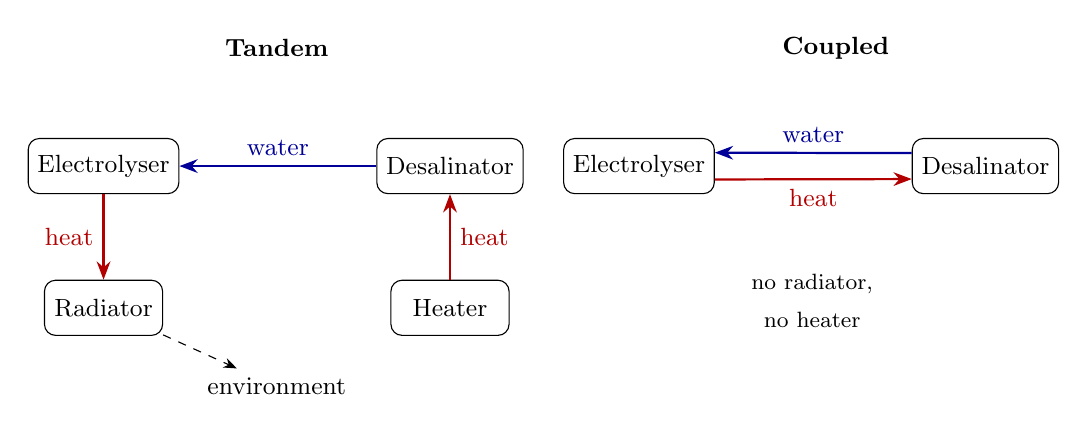
\begin{tikzpicture}[>=Stealth,every node/.style={font=\small},
  proc/.style={draw,rounded corners,minimum width=1.5cm,minimum height=0.7cm}]
  % tandem
  \node at (2.2,2.4) {\textbf{Tandem}};
  \node[proc] (E1) at (0,0.9) {Electrolyser};
  \node[proc] (D1) at (4.4,0.9) {Desalinator};
  \node[proc] (R1) at (0,-0.9) {Radiator};
  \node[proc] (H1) at (4.4,-0.9) {Heater};
  \node (X1) at (2.2,-1.9) {environment};
  \draw[->,thick,blue!60!black] (D1) -- node[above]{water} (E1);
  \draw[->,thick,red!70!black] (E1) -- node[left]{heat} (R1);
  \draw[->,thick,red!70!black] (H1) -- node[right]{heat} (D1);
  \draw[->,dashed] (R1) -- (X1);
  % coupled
  \begin{scope}[xshift=8.4cm]
  \node at (0.9,2.4) {\textbf{Coupled}};
  \node[proc] (E2) at (-1.6,0.9) {Electrolyser};
  \node[proc] (D2) at (2.8,0.9) {Desalinator};
  \draw[->,thick,blue!60!black] (D2.170) -- node[above]{water} (E2.10);
  \draw[->,thick,red!70!black] (E2.350) -- node[below]{heat} (D2.190);
  \node at (0.6,-0.6) {\footnotesize no radiator,};
  \node at (0.6,-1.05) {\footnotesize no heater};
  \end{scope}
\end{tikzpicture}
\caption{Residual graphs of the paper's tandem control and coupled system, with the desalination process held identical. The coupled graph contains a two-cycle: each process supplies the other. The tandem graph is acyclic and sends the electrolyser's heat to the environment.}
\label{fig:graphs}
\end{figure}

Two structural features are worth stating. First, the coupled graph contains a cycle. The electrolyser supplies the desalinator with heat, the desalinator supplies the electrolyser with water, and the flows are of different kinds. The circular-economy image of a chain in which each process feeds the next understates this. Second, the exchange sets a constraint that is an opportunity: the electrolyser must reject heat at a rate that keeps it near 85\,$^{\circ}$C (the paper holds it to $\pm1\,^{\circ}$C by a branch valve that sets the share of lye passed through the desalination heat exchanger), and the desalinator needs heat at a rate that depends on how much water is wanted. The design works because one requirement's magnitude falls inside the other's demand. Write the residual set of $A$ as $\mathcal{R}_A$ and the demand set of $B$ as $\mathcal{D}_B$. The processes are complementary when $\mathcal{R}_A\cap\mathcal{D}_B\neq\varnothing$.

A tempting formalization is to search over graphs for the one maximizing a sum of pairwise compatibilities, $\sum_{(i,j)\in E}\operatorname{compat}(\mathcal{R}_i,\mathcal{D}_j)$. That objective is incomplete, and the paper shows why. A useful topology objective is net system performance,
\[
  J(G) \;=\; \text{useful output}(G)\;-\;\text{input}(G)\;-\;\text{coupling cost}(G),
\]
where the coupling cost includes lost degrees of freedom. In the coupled plant the water output is slaved to the hydrogen output, since both depend on the electrolyser's load; the paper's Figure~4e shows co-productivity of fresh water rising with hydrogen productivity, and reports operation under daily start-stop cycles. In a tandem plant the desalinator could run on its own schedule. This is the essay's inference from the paper's data and not a finding of the paper, but it belongs in the accounting: a topology that closes a residual loop also ties two schedules together.

\section{The better component}

The paper contains one qualification that the essay's argument turns on. It states that the efficiency improvement depends on the amount of waste heat generated, and that for electrolysers of higher electrical efficiency the waste heat would be lower and the corresponding improvement in system electrical efficiency would diminish. A more efficient component reduces the value of a coupling designed around its inefficiency.

The dependence can be made explicit. Since $\eta_{\mathrm{electrolyser}}=\Et/\Ep$ and $\dot Q_{\mathrm{WH}}=\Ep(1-\eta)\dot V_{\mathrm{H_2}}$, the waste heat per normal cubic metre is
\begin{equation}
  \QWH \;=\; \Ep-\Et,
  \label{eq:qwh}
\end{equation}
with $\Et=3.52\,\mathrm{kWh\,Nm^{-3}}$ at 85\,$^{\circ}$C. The paper's regulated-load figure (Fig.~4d) shows exactly this line: waste heat output rising from about 0.47 to about 0.88\,kWh\,Nm$^{-3}$ as the electrolyser's consumption rises from 4.0 to 4.4.

The water demand of electrolysis is met from the heat. With a total heat of vaporization of about 0.70\,kWh\,kg$^{-1}$ near 50\,$^{\circ}$C (the paper gives 0.68 to 0.71), the 0.8\,kg of water needed per normal cubic metre requires about 0.56\,kWh. The required utilization rate is therefore
\begin{equation}
  u_{\min}(\QWH)\;=\;\frac{0.56}{\QWH},
  \label{eq:umin}
\end{equation}
which reproduces the paper's stated figures: 56\,\% at 1.0\,kWh\,Nm$^{-3}$ and 37\,\% at 1.5. Figure~\ref{fig:umin} plots the requirement. It rises without bound as heat output falls, and reaches 100\,\% at $\QWH=0.56$, that is at $\Ep\approx4.08$\,kWh\,Nm$^{-3}$. At the paper's measured utilization of about 85\,\% the corresponding electrolyser consumption is near 4.18. Below it, the heat of a better electrolyser cannot supply the electrolyser's own water at this boiling temperature.

\begin{figure}[t]
\centering
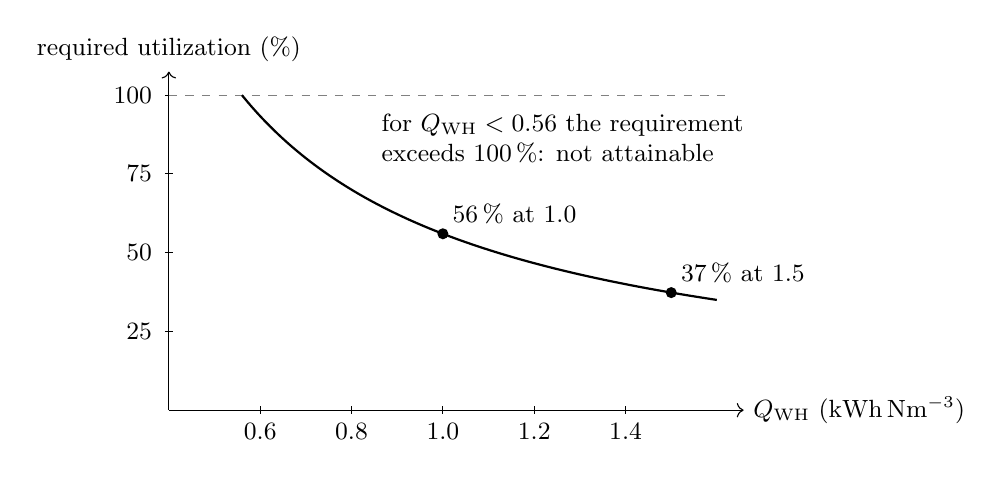
\begin{tikzpicture}[scale=1.0]
  \draw[->] (0.3,0) -- (7.6,0) node[right] {\small $\QWH$ (kWh\,Nm$^{-3}$)};
  \draw[->] (0.3,0) -- (0.3,4.3) node[above] {\small required utilization (\%)};
  % axis x from 0.4 to 1.6 mapped: x = 0.3 + (Q-0.4)*5.8 ; y = u*0.04
  \foreach \q/\x in {0.6/1.46,0.8/2.62,1.0/3.78,1.2/4.94,1.4/6.10} {
     \draw (\x,0.05) -- (\x,-0.05) node[below] {\small \q};
  }
  \foreach \y/\l in {1/25,2/50,3/75,4/100} {
     \draw (0.25,\y) -- (0.35,\y) node[left,xshift=-4pt] {\small \l};
  }
  \draw[dashed,gray] (0.3,4) -- (7.4,4);
  % curve u = 0.56/Q *100 % -> y = 0.04*56/Q = 2.24/Q ; Q from 0.56 to 1.6
  \draw[thick,domain=0.56:1.6,samples=60,smooth] plot ({0.3+(\x-0.4)*5.8},{2.24/\x});
  \fill (3.78,2.24) circle (2pt) node[above right] {\small 56\,\% at 1.0};
  \fill (6.68,1.493) circle (2pt) node[above right] {\small 37\,\% at 1.5};
  \node[align=left,font=\small] at (5.3,3.45) {for $\QWH<0.56$ the requirement\\ exceeds 100\,\%: not attainable};
\end{tikzpicture}
\caption{Utilization of waste heat needed for the electrolyser to supply its own water at a boiling temperature near 50\,$^{\circ}$C, from Equation~\eqref{eq:umin}. The two labelled points are the figures stated in the paper.}
\label{fig:umin}
\end{figure}

This is the sense in which the component derivative is not the system derivative. Let $J$ be a system objective in electricity-equivalent units that credits exported fresh water at a value $v$ per kilogram, and write $h$ for the heat of vaporization per kilogram. In the regime where the heat exceeds the self-supply requirement, the exported water is $m_w=[\kappa(\Ep-\Et)/h-0.8]$ kilograms per normal cubic metre, so
\begin{equation}
  J \;=\; \Ep - v\,m_w, \qquad
  \frac{\partial J}{\partial \Ep} \;=\; 1-\frac{v\,\kappa}{h}.
  \label{eq:derivative}
\end{equation}
The component derivative, $\partial \Ep/\partial \Ep=1$, is the electricity saved by a better electrolyser. The system derivative subtracts the co-product income that the improvement removes. It is smaller, and it changes sign only if $v>h/\kappa\approx0.8$\,kWh per kilogram, which at electricity prices of a few cents per kilowatt-hour corresponds to a water value on the order of tens of dollars per cubic metre. That is far above the price of desalinated water, so in ordinary circumstances a better electrolyser still improves the coupled system, and what erodes is the margin the coupling holds over an uncoupled plant, which is precisely what the paper reports. The essay's point is structural. Once a subsystem has been built to consume another's residual, improvements to the source are not evaluated independently of the sink, and in a heat-limited regime the correction is large: if the heat had to be replaced by resistive heating at unit cost, the term $v\kappa/h$ would be replaced by $\kappa$, and about 85\,\% of an electrolyser's efficiency gain would be offset in that regime.

\section{Waste as a relation}

The definition of Section~2 can be written as a predicate with its qualifications displayed. Instead of $\operatorname{Waste}(x)$, the accurate form is
\[
  \operatorname{Waste}(x\mid S,t,\mathcal{O}),
\]
meaning that $x$ has no admitted continuation within system $S$, at time $t$, under the available operations $\mathcal{O}$. Each argument is something the paper changes. It moves the boundary $S$ by internalizing the desalinator, and it enlarges $\mathcal{O}$ by using a vacuum evaporator, which exposes a low-temperature sink. The heat is unchanged in temperature and quantity.

The same form clarifies what a refusal is. A residual that is rejected by one continuation, here heat at 85\,$^{\circ}$C refused by an atmospheric-pressure evaporator, need not be rejected by another, here a reduced-pressure one. Refusal is indexed by the continuation. This is consistent with the two earlier essays of this series. In \emph{When Failure Becomes a Signal}, an obstruction is converted into information that changes what is next admissible. In \emph{The Unequal Error}, the seriousness of an error is fixed by what it can later corrupt. Here, the classification of a flow as waste is fixed by what can be done with it next. The common structure is that a residue, an error, or a refusal is intelligible only relative to the continuations available downstream. A related pattern is temporal: accumulation that is a residue at one time scale can be a substrate at another, as in a berm or a soil built from what was discarded. The heat exchange here is the immediate counterpart of that slower case, $\text{residual}_t\to\text{condition of production}_{t+1}$ in a single operating cycle. These connections are offered as a reading and not as evidence for any framework; the paper is an independent engineering result that happens to display the structure.

The general proposition the essay supports is a qualified one:
\begin{quote}
\emph{Waste is a relation between a stream and a system boundary. There are streams whose continuations lie outside the chosen system, and streams for which no continuation exists at any boundary. The word ``waste'' conflates the two.}
\end{quote}
Irreversibility remains real. Nothing here says that everything can be recycled indefinitely, and the paper's own 15\,\% remainder and the low work potential of its heat say otherwise.

\section{Where the evidence stops}

\begin{itemize}[leftmargin=1.6em,itemsep=2pt]
  \item \textbf{Duration and load profile.} The pilot ran 100 days and the demonstration 40 days, both under daily start-stop operation with a 4-hour steady load. This is short of the multi-year operation an industrial plant would need, and continuous operation was not tested. Membrane-free vacuum distillation avoids the wetting and fouling of membrane distillation, but fouling of the exchanger by seawater over long periods is not addressed beyond the material choice.
  \item \textbf{Scale and single-stage operation.} The 250\,kW unit uses a single-stage distillation. The paper states that an industrial-scale system would need multi-stage distillation to recover the heat, and the economic comparison is a modelled plant of 50 tonnes of hydrogen and 9,285 tonnes of fresh water per day, not a measured one. The water produced by the demonstration is small: 31.6\,kg\,h$^{-1}$ net.
  \item \textbf{The efficiency metric depends on the boundary.} The reported improvements of 9.0\,\%, 12.5\,\%, and 14.4\,\% are differences between two efficiencies (Equation~22), each defined with the heat used for vaporization counted as useful output. The figures are percentage points of this metric, not fractions of a baseline consumption, and they measure a comparison between two configurations under one convention. The essay's own back-of-envelope calculation from the main-text inputs (waste heat, utilization, vaporization heat, electrolyser consumption) gave larger gains than those reported, presumably because auxiliary loads are itemized only in the supplementary information. The reported values are used here as stated.
  \item \textbf{Economics are preliminary and the margin over reverse osmosis is small.} The paper describes its techno-economic analysis as preliminary. Against the tandem reverse osmosis system it finds total energy about 5\,\% lower and a levelized cost of hydrogen 6 to 9\,\% lower at electricity prices of US\$0.01 to 0.05 per kilowatt-hour. The advantage over the multi-effect distillation tandem is larger. The stated levelized costs, US\$2.1 and US\$2.9 per kilogram, assume a capacity factor of 97\,\% and depend strongly on electricity prices.
  \item \textbf{Brine.} The paper describes the concentrated brine as a resource, with recovery of salt, uranium, and bromine as possibilities. Recovery is not demonstrated, and in the paper's accounting the brine discharge is one of the pathways that carries heat away.
  \item \textbf{The derivations here are first order.} Equations~\eqref{eq:umin} and \eqref{eq:derivative} follow from figures the paper states, with $h\approx0.70$\,kWh\,kg$^{-1}$ and idealized utilization. They sit uneasily with the small positive co-production the paper reports at the lowest loads (Fig.~4e), where waste heat output falls near or below the self-supply threshold, and should be checked against the supplementary data. The work-potential figures assume an ambient near 15\,$^{\circ}$C, a value the paper does not give.
\end{itemize}

\section{Conclusion}

The paper's system is a plant in which the cooling load and the heating load are one heat exchange, and its important result for theory is that the exchange is made possible by changing the sink and not the source. The residue, 80 to 90\,$^{\circ}$C heat, was never made better. The evaporator was made to accept it by lowering the pressure at which water boils, and the desalinator was moved inside the boundary so that its demand and the electrolyser's obligation could meet. The measured benefit of doing so, holding the desalination process fixed, is 17.7\,\% of the energy consumption of the uncoupled arrangement.

Three lessons follow. Waste is a relation among a stream, a boundary, and a set of operations, and can be changed by changing any of them. A residual that fails to meet a sink can be treated by transforming the sink, at a price that reappears as a new constraint elsewhere in the process. And once a sink is built around a residual, the source can no longer be improved without regard to the sink: the electrolyser's efficiency is a component property, the value of its inefficiency is a property of the topology, and efficiency, in this case, is partly a property of how the parts are connected.

\begin{thebibliography}{9}
\bibitem{jiang2026} S.~Jiang, P.~Zhu, Y.~Liu and D.~Deng, A 250-kilowatt system for co-production of hydrogen and fresh water from seawater, \emph{Nat.\ Energy} (2026), \url{https://doi.org/10.1038/s41560-026-02130-6}.
\bibitem{stull} D.~R.~Stull, Vapor pressure of pure substances, organic and inorganic compounds, \emph{Ind.\ Eng.\ Chem.}\ \textbf{39}, 517--550 (1947).
\bibitem{horseman} T.~Horseman \emph{et al.}, Wetting, scaling, and fouling in membrane distillation: state-of-the-art insights on fundamental mechanisms and mitigation strategies, \emph{ACS ES\&T Eng.}\ \textbf{1}, 117--140 (2020).
\end{thebibliography}

\end{document}
